\documentclass[aspectratio=169,11pt]{beamer}
\usepackage[T1]{fontenc}
\usepackage{lmodern,amsmath,amssymb,mathtools,bm,booktabs,array,graphicx,tikz}
\usetikzlibrary{arrows.meta,positioning,calc,decorations.pathreplacing,patterns}
\definecolor{ink}{HTML}{17344D}\definecolor{accent}{HTML}{087E8B}\definecolor{pale}{HTML}{EDF5F5}\definecolor{gold}{HTML}{AD6B19}
\providecommand{\dd}{\,\mathrm{d}}\providecommand{\R}{\mathbb{R}}
\providecommand{\E}{\mathbb{E}}\providecommand{\Var}{\operatorname{Var}}
\providecommand{\Cov}{\operatorname{Cov}}\providecommand{\diag}{\operatorname{diag}}
\providecommand{\norm}[1]{\left\lVert#1\right\rVert}
\providecommand{\abs}[1]{\left|#1\right|}
\usefonttheme{professionalfonts}
\setbeamercolor{normal text}{fg=black,bg=white}
\setbeamercolor{frametitle}{fg=ink,bg=white}
\setbeamercolor{title}{fg=ink}\setbeamercolor{structure}{fg=accent}
\setbeamercolor{block title}{fg=ink,bg=pale}\setbeamercolor{block body}{fg=black,bg=pale!40}
\setbeamercolor{alerted text}{fg=accent}
\setbeamerfont{frametitle}{size=\Large,series=\bfseries}
\setbeamerfont{title}{size=\LARGE,series=\bfseries}
\setbeamertemplate{navigation symbols}{}
\setbeamersize{text margin left=.7cm,text margin right=.7cm}
\setbeamertemplate{frametitle}{\vspace{.18cm}\insertframetitle\par\vspace{.1cm}{\color{accent}\hrule height .6pt}\vspace{.12cm}}
\newcommand{\notestarget}{notes.pdf}\newcommand{\noteslabel}{Notes}
\setbeamertemplate{footline}{\hspace{.7cm}\color{ink}\scriptsize Mathematical Cardiology\quad\href{\notestarget}{\noteslabel}\hfill\insertframenumber\,/\,\inserttotalframenumber\hspace{.7cm}\vspace{.18cm}}
\setbeamercovered{invisible}
\hypersetup{pdfauthor={Zan Ahmad},pdftitle={Calibrating a flow law and constructing a classifier},pdfpagemode=UseNone}
\begin{document}
\begin{frame}[plain]\vfill
{\small\color{accent} Mathematical Cardiology \quad Lecture 8}\par\medskip
{\raggedright\hyphenpenalty=10000\exhyphenpenalty=10000\LARGE\bfseries\color{ink} Calibrating a flow law and constructing a classifier}\par\bigskip
Zan Ahmad\par\smallskip
{\small Fall 2023}\par\vfill\end{frame}
\renewcommand{\notestarget}{notes.pdf\#note-a-passive-law-with-an-unknown-coefficient}
\begin{frame}[label=slide-a-parameter-inside-a-physical-relation-figure]{A parameter inside a physical relation}
\centering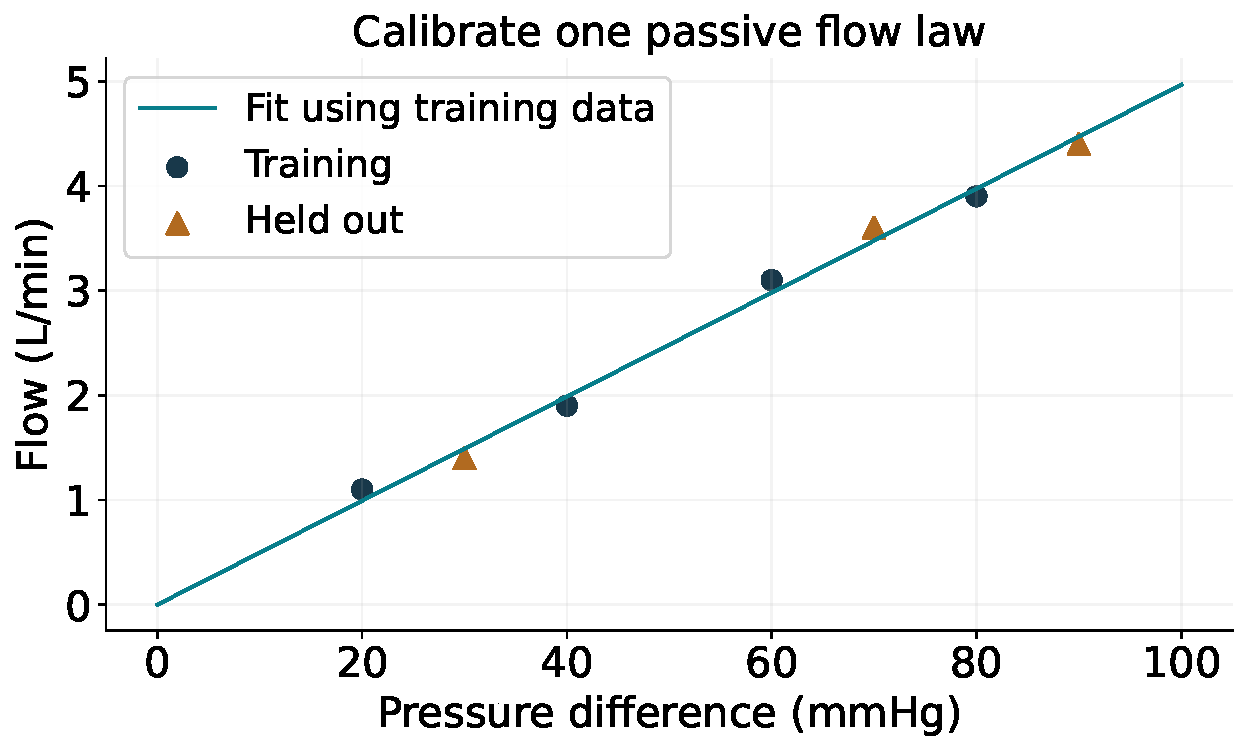
\includegraphics[width=.98\linewidth,height=.69\textheight,keepaspectratio]{calibration.pdf}\end{frame}
\renewcommand{\notestarget}{notes.pdf\#note-a-passive-law-with-an-unknown-coefficient}
\begin{frame}[t,fragile,label=slide-a-parameter-inside-a-physical-relation]{A parameter inside a physical relation}
\[\widehat Q=G\Delta P,\qquad R=1/G.\]
$G$ has units $\mathrm{L/(min\,mmHg)}$.
\pause{}
A line through the origin asserts zero passive flow at equal boundary pressures.
\end{frame}
\renewcommand{\notestarget}{notes.pdf\#note-least-squares-without-differentiation}
\begin{frame}[t,fragile,label=slide-define-the-discrepancy]{Define the discrepancy}
For training pairs $(x_i,y_i)$,
\[r_i(G)=Gx_i-y_i,\qquad S(G)=\sum_i r_i(G)^2.\]
\pause{}
Opposite signed errors do not cancel after squaring.
The objective has units $(\mathrm{L/min})^2$.
\end{frame}
\renewcommand{\notestarget}{notes.pdf\#note-least-squares-without-differentiation}
\begin{frame}[t,fragile,label=slide-expand-the-objective]{Expand the objective}
\[S(G)=\sum_i(G^2x_i^2-2Gx_iy_i+y_i^2).\]
\pause{}
Write
\[S(G)=AG^2-2BG+C,\]
where $A=\sum x_i^2$, $B=\sum x_iy_i$, $C=\sum y_i^2$.
\end{frame}
\renewcommand{\notestarget}{notes.pdf\#note-least-squares-without-differentiation}
\begin{frame}[t,fragile,label=slide-complete-one-square]{Complete one square}
When $A>0$,
\[S(G)=A(G-B/A)^2+C-B^2/A.\]
\pause{}
The square is smallest at zero, so
\[\boxed{\widehat G=B/A}.\]
\end{frame}
\renewcommand{\notestarget}{notes.pdf\#note-least-squares-without-differentiation}
\begin{frame}[t,fragile,label=slide-evaluate-the-fitted-conductance]{Evaluate the fitted conductance}
For the four displayed training observations,
\[A=12000,\qquad B=596.\]
\pause{}
\[\widehat G=0.049667,\qquad\widehat R=20.134\,\mathrm{mmHg\,min/L}.\]
These digits describe this synthetic sample.
\end{frame}
\renewcommand{\notestarget}{notes.pdf\#note-least-squares-without-differentiation}
\begin{frame}[t,fragile,label=slide-an-experiment-with-no-slope-information]{An experiment with no slope information}
If every training pressure difference is zero,
\[A=0,\qquad S(G)=\sum_i y_i^2.\]
\pause{}
Every $G$ gives the same objective.
More zero-pressure observations do not identify conductance.
\end{frame}
\renewcommand{\notestarget}{notes.pdf\#note-least-squares-without-differentiation}
\begin{frame}[t,fragile,label=slide-a-unit-conversion-check]{A unit conversion check}
Let $x'_i=cx_i$ with $c>0$.
\[\widehat G'=\frac{c\sum x_iy_i}{c^2\sum x_i^2}=\widehat G/c.\]
\pause{}
\[\widehat G'x'_i=\widehat Gx_i.\]
The prediction stays the same.
\end{frame}
\renewcommand{\notestarget}{notes.pdf\#note-a-frozen-rule-on-new-observations}
\begin{frame}[t,fragile,label=slide-evaluate-the-frozen-line]{Evaluate the frozen line}
\[
\begin{array}{c|rrr}
x&30&70&90\\\hline
y&1.4&3.6&4.4\\
\widehat y&1.4900&3.4767&4.4700\\
r&0.0900&-0.1233&0.0700
\end{array}
\]
\pause{}
$\operatorname{MAE}\simeq0.09444\,\mathrm{L/min}$.
\end{frame}
\renewcommand{\notestarget}{notes.pdf\#note-a-frozen-rule-on-new-observations}
\begin{frame}[t,fragile,label=slide-compare-with-a-constant-predictor]{Compare with a constant predictor}
The training mean is $2.5\,\mathrm{L/min}$.
\pause{}
Its held-out absolute errors are $1.1$, $1.1$, $1.9$.
\[\operatorname{MAE}_{\rm constant}=4.1/3\simeq1.3667\,\mathrm{L/min}.\]
Both rules are evaluated on the same three cases.
\end{frame}
\renewcommand{\notestarget}{notes.pdf\#note-training-coordinates-and-class-centers}
\begin{frame}[label=slide-fit-a-coordinate-system-on-training-cases-figure]{Fit a coordinate system on training cases}
\centering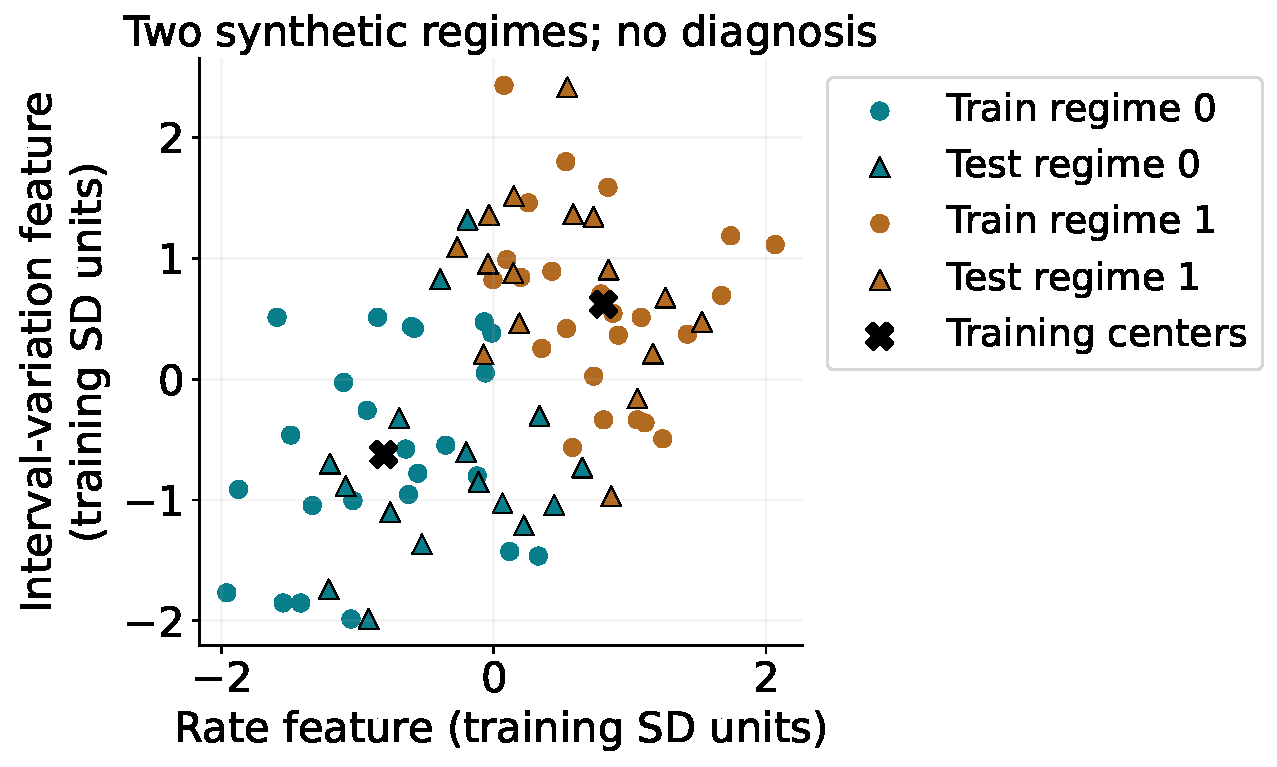
\includegraphics[width=.98\linewidth,height=.69\textheight,keepaspectratio]{classification.pdf}\end{frame}
\renewcommand{\notestarget}{notes.pdf\#note-training-coordinates-and-class-centers}
\begin{frame}[t,fragile,label=slide-fit-a-coordinate-system-on-training-cases]{Fit a coordinate system on training cases}
For each feature,
\[z_j=(x_j-\mu_j)/s_j.\]
\pause{}
Compute $\mu_j,s_j$ from the 48 training cases.
Use those same values for the 32 held-out cases.
\end{frame}
\renewcommand{\notestarget}{notes.pdf\#note-training-coordinates-and-class-centers}
\begin{frame}[t,fragile,label=slide-the-nearer-training-center]{The nearer training center}
Let $c_0,c_1$ be the class means in standardized coordinates.
\[d_k(z)=\sum_{j=1}^2(z_j-c_{kj})^2.\]
\pause{}
Choose the smaller $d_k$; exact ties go to zero in this implementation.
\end{frame}
\renewcommand{\notestarget}{notes.pdf\#note-the-boundary-hidden-in-the-distance-comparison}
\begin{frame}[t,fragile,label=slide-expand-the-decision-boundary]{Expand the decision boundary}
Label one requires
\[\|z-c_1\|^2<\|z-c_0\|^2.\]
\pause{}
The $\|z\|^2$ terms cancel:
\[2z\cdot(c_1-c_0)>\|c_1\|^2-\|c_0\|^2.\]
Equality is a line when the centers differ.
\end{frame}
\renewcommand{\notestarget}{notes.pdf\#note-the-boundary-hidden-in-the-distance-comparison}
\begin{frame}[t,fragile,label=slide-scaling-determines-the-metric]{Scaling determines the metric}
In raw coordinates,
\[d_k(x)=\sum_{j=1}^2\frac{(x_j-\overline x_{kj})^2}{s_j^2}.\]
\pause{}
The training variations determine the weights.
A new test mean would change the fitted rule.
\end{frame}
\renewcommand{\notestarget}{notes.pdf\#note-count-the-errors-the-claim-actually-concerns}
\begin{frame}[t,fragile,label=slide-read-both-directions-of-error]{Read both directions of error}
\[
\begin{array}{c|rr}
\text{true}\backslash\text{predicted}&0&1\\\hline
0&12&4\\
1&0&16
\end{array}
\]
\pause{}
Accuracy is $28/32=0.875$.
All four errors are $0\to1$.
\end{frame}
\renewcommand{\notestarget}{notes.pdf\#note-count-the-errors-the-claim-actually-concerns}
\begin{frame}[t,fragile,label=slide-the-held-out-unit-belongs-to-the-claim]{The held-out unit belongs to the claim}
A claim about new people requires whole people to be held out.
\pause{}
Windows from one person can share information even if the windows differ.

Choose the grouping first; fit scaling and the rule on training groups.
\end{frame}
\renewcommand{\notestarget}{notes.pdf\#note-count-the-errors-the-claim-actually-concerns}
\begin{frame}[t,fragile,label=slide-after-inspecting-an-error]{After inspecting an error}
Changing the model in response to test errors makes those cases development data.
\pause{}
Retain the original result. Evaluate the changed rule on other observations.

A transparent fit is useful because its assumptions and failures can be named.
\end{frame}
\end{document}
